\documentclass{article}
\usepackage[utf8]{inputenc}
\usepackage{graphicx}
\usepackage{xcolor}
\usepackage{fancyhdr}
\usepackage[greek,english]{babel}
\usepackage{alphabeta}
\usepackage{listings}
\usepackage{caption}
\usepackage{float}
\usepackage{minted}
\usepackage{enumitem}
\usepackage{array}


\usepackage{hyperref}
\hypersetup{
    colorlinks=true,
    linkcolor=blue,
    filecolor=magenta,
    urlcolor=cyan,
}

\usepackage{geometry}
 \geometry{
 a4paper,
 total={170mm,257mm},
 left=20mm,
 top=20mm,
 }

\lstset{
  basicstyle=\ttfamily,
  showstringspaces=false,
  commentstyle=\color{red},
  keywordstyle=\color{blue},
  backgroundcolor = \color{lightgray},
  breaklines
}
\definecolor{LightGray}{rgb}{71,68,68}

\graphicspath{{images}}

\pagestyle{fancy}
\lhead{X Εργασία Μαθήματος }
\rhead{\thepage}
\cfoot{Ταύρος, 22 Ιανουαρίου 2020, Όνομα Φοιτητή, Μάθημα , Χ Εργασία }
\renewcommand{\headrulewidth}{0.4pt}
\renewcommand{\footrulewidth}{0.4pt}

\begin{document}

\begin{titlepage}
\centering
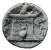
\includegraphics{/logo.png} % University logo %
\par
\Huge{Χαροκόπειο Πανεπιστήμιο}
\par
\LARGE{Τμήμα Πληροφορικής και Τηλεματικής}
\par
\vspace{1cm}
\huge{Εργασία στο μάθημα Χ}
\vspace{1cm}
\par
\huge{Όνομα Φοιτητή}
\par
(ΑΜ Φοιτητή)
\par
\vspace{1cm}
\large{Ταύρος, 22 Ιανουαρίου 2020}

\end{titlepage}


\newpage
%----- "CONTENTS" PAGE ------------
\Huge{Περιεχόμενα}
\par
\vspace{1cm}
\huge{1. ΘΕΜΑ Α}
\makeatletter
\newcommand\cdotfill{%
    \leavevmode\cleaders\hb@xt@.44em{\hss$\cdot$\hss}\hfill\kern\z@
}
\makeatother
\Large{
\begin{enumerate}[align=parleft]
  \item[1.1] Ζητούμενο \cdotfill 2
  \item[1.2] Λογική  \cdotfill 2
  \item[1.3] Κώδικας  \cdotfill 2
  \item[1.4] Ενδεικτικές εκτελέσεις (screenshots) \cdotfill 4
  \item[1.5] Γενικά σχόλια/παρατηρήσεις \cdotfill 4
\end{enumerate}
}
%
\par
\vspace{1cm}
\huge{2. ΘΕΜΑ Β}
\makeatletter

\makeatother
\Large{
\begin{enumerate}[align=parleft]
  \item[2.1] Λογική  \cdotfill 5
  \item[2.2] Κώδικας \cdotfill 5
  \item[2.3] Ενδεικτικές εκτελέσεις (screenshots) \cdotfill 10
  \item[2.4] Γενικά σχόλια/παρατηρήσεις \cdotfill 12
\end{enumerate}
}
%
\par
\vspace{1cm}
\huge{3. ΘΕΜΑ Γ}
\makeatletter

\makeatother
\Large{
\begin{enumerate}[align=parleft]
  \item[3.1] Λογική  \cdotfill 13
  \item[3.2] Κώδικας \cdotfill 13
\end{enumerate}
}
%
\par
\vspace{1cm}
\huge{ 4. ΘΕΜΑ Δ}
\makeatletter
\makeatother
\Large{
\begin{enumerate}[align=parleft]
  \item[4.1] Compile from source και makefile \cdotfill 15
\end{enumerate}
}
\par
\vspace{1cm}
%
\huge{5. ΘΕΜΑ Ε}
\makeatletter

\makeatother
\Large{
\begin{enumerate}[align=parleft]
  \item[5.1] Σχόλια, συνοπτικός πίνακας και δυσκολίες \cdotfill 15
\end{enumerate}
}


%------ END OF "CONTENTS" PAGE ----


%------------ PAGE START -----------
\newpage

\Huge{1. Γενικός τίτλος}
\par
\vspace{0.5cm}
\huge{1.1 Ζητούμενο}
\par
\vspace{0.4cm}
\large{Ζητούμενο ....}

\vspace{0.4cm}

\huge{1.2 Λογική }

\vspace{0.4cm}

\large{Η λογική .... }
\par
\vspace{0.5cm}
\huge{1.3 Κώδικας }

%---- CODE START ---
\begin{minted}[fontsize=\normalsize,bgcolor=lightgray]{c}
#include <stdio.h>
int main(int argc, char **argv{
    return 0;
}
\end{minted}
%---- CODE END ----

\huge{1.4 Ενδεικτικές εκτελέσεις (screenshots):}

\begin{center}
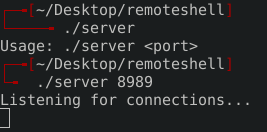
\includegraphics[width=10cm,height=5cm,keepaspectratio]{/listenmode.png}
\captionof{figure}{Server σε listen mode.}
\end{center}


\huge{1.5 Γενικά σχόλια/παρατηρήσεις:}
\par
\vspace{0.5cm}
\large{
\par
Ο τερματισμός του server γίνεται με την χρήση του σήματος SIGINT από το πληκτρολόγιο και εμφανίζεται αντίστοιχο μήνυμα στην οθόνη.
\par
}
\vspace{0.5cm}
\begin{center}
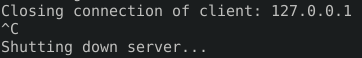
\includegraphics[width=10cm,height=5cm,keepaspectratio]{/shutdownservre.png}
\captionof{figure}{Τερματισμός server.}
\end{center}
%------------ PAGE END -------------


\par
\vspace{0.2cm}


\par
\vspace{1cm}
\centering
\begin{tabular}{ |p{13cm}||p{3cm}|  }
 \hline
 \multicolumn{2}{|c|}{2η Εργασία} \\
 \hline
 & Υλοποιήθηκε\\
 \hline

ΖΗΤΟΥΜΕΝΟ 1
   & ΝΑΙ    \\
 ΖΗΤΟΥΜΕΝΟ 2&   ΝΑΙ  \\
 ΖΗΤΟΥΜΕΝΟ 3 &ΝΑΙ \\
 ΖΗΤΟΥΜΕΝΟ 4
    &ΝΑΙ \\
 ΖΗΤΟΥΜΕΝΟ 5&   ΝΑΙ  \\
 ΖΗΤΟΥΜΕΝΟ 6& NAI    \\
 ΖΗΤΟΥΜΕΝΟ 7& ΝΑΙ  \\
 \hline
\end{tabular}
%------------ PAGE END -------------
\end{document}
